% % \begin{table}[H]
% %   \begin{NiceTabular}{ccccccccc}[vlines] % <-- 9 columns now (was 7)
% %    \Hline
% %    \Block{1-2}{\diagbox{\enskip \textbf{Examples}}{\textbf{Techniques}}} & &
% %    \RowStyle{\rotate}
% %     \makecell{Forward\\ closure \\~\cite{Plump1995}} % NEW column #1
% %    & \RowStyle{\rotate}
% %     \makecell{Modular \\ criterion \\~\cite{plump2018modular}} % NEW column #2
% %    & \RowStyle{\rotate}
% %     \makecell{Type graph \\~\cite{bruggink2014termination}}  
% %    & \RowStyle{\rotate}
% %     \makecell{Type graph \\~\cite{bruggink2015proving}} 
% %    & \RowStyle{\rotate}
% %     \makecell{Type graph \\~\cite{endrullis2024generalized_arxiv_v2}} 
% %    & \RowStyle{\rotate}
% %     \makecell{Subgraph \\counting \\~\cite{overbeek2024termination_lmcs}}
% %    & \RowStyle{\rotate}
% %     \makecell{Our proposal} \\
% %    \Hline
% %    \Hline
% %    % ----- from plump 1995 -----
% %    \Block{2-1}{\cite{Plump1995}} 
% %     & \hyperref[ex:overbeek_5d8_plump1995_3d8_plump2018_3_overbeek_5d8]{Example 3.8} 
% %                  & \ding{51} & -- & -- & -- & -- &\ding{51} & \ding{51}\\ 
% %     \Hline
% %     & Example 4.1 & \ding{51} & -- & -- & -- & -- & \ding{51}& \ding{55}\\ 
% %     \hline
% %     % ----- from plump 2018 -----
% %    \Block{4-1}{\cite{plump2018modular}} 
% %    & \hyperref[ex:overbeek_5d8_plump1995_3d8_plump2018_3_overbeek_5d8]{Example 3} 
% %               & -- & \ding{51} &  -- & -- & -- & \ding{51} & \ding{51}\\ 
% %    \Hline
% %    & \hyperref[ex:plump_ex4]{Example 4} &  -- &  \ding{51} &  -- & -- & -- & \ding{55} &\ding{55}\\ 
% %    \Hline
% %    & Example 5 &  -- &  \ding{51} &   -- & -- & -- &  \ding{51} & \ding{51}\\ 
% %    \Hline
% %    & Example 6 s->s&  -- & \ding{51} & -- & -- & -- & \ding{51} & \ding{55}\\ 
% %    \Hline
% %    % ----- from bruggink2014 -----
% %    \Block{4-1}{\cite{bruggink2014termination}} 
% %     & Example 1 
% %       & -- & -- & \ding{51} & -- & -- & \ding{55} & \ding{55}\\ \Hline
% %    & \hyperref[ex:plump_ex4]{Example 5}
% %       & -- & -- & \ding{51} & -- & -- & -- &  \ding{55}\\ \Hline
% %    & \hyperref[ex:termination:grsaa]{Example 4 and 6}  grsaa
% %       & -- & -- & \ding{51} & -- & -- & ? & \ding{51} \\ \Hline
% %    & Routing Protocol
% %       & -- & -- & \ding{51} & -- & -- & \ding{55} &  \ding{55}\\ \Hline
% %    %~\autoref{ex_contrib_variant} 
% %    %   & \ding{55} & -- & -- & -- & \ding{51}\\ \Hline
   
% %    % ----- from bruggink2015 -----
% %    \Block{4-1}{\cite{bruggink2015proving}}
% %     &\hyperref[ex:termination:grsaa]{Example 2} grsaa
% %       & -- & -- & -- & \ding{51} & -- & ? &  \ding{51}\\ \Hline
% %    & Example 4 
% %       & -- & -- & -- & \ding{51} & -- & \ding{51} & \ding{51} \\ \Hline
% %    & Example 5 
% %       & -- & -- & -- & \ding{51} & -- & \ding{55} & \ding{55}\\ \Hline
% %    & Example 6 
% %       & -- & -- & -- & \ding{51} & -- & \ding{55} & \ding{55}\\ \Hline
% %    %~\autoref{ex_contrib_variant} 
% %    %   & -- & \ding{55} & -- & -- & \ding{51}\\ \Hline
   
% %    % ----- from endrullis2024generalized_arxiv_v2 -----
% %    \Block{8-1}{\cite{endrullis2024generalized_arxiv_v2}}
% %     & Example 6.2  
% %       & -- & -- & -- & -- & \ding{51} & -- & \ding{51}\\ \Hline
% %    & \hyperref[ex_endrullis_5d8_overbeek]{Example 6.3}
% %       & -- & -- & -- & -- & \ding{51} & \ding{55} & \ding{51}\\ \Hline
% %    & Example 6.4 SGraph
% %       & -- & -- & -- & -- & -- & -- & -- \\ \Hline
% %    & Example 6.5  SGraph
% %       & -- & -- & -- & -- &  -- & -- & -- \\ \Hline
% %    & \hyperref[ex:overbeek_5d8_plump1995_3d8_plump2018_3_overbeek_5d8]{Example D.1}
% %       & -- & -- & -- & -- & \ding{51} & -- & \ding{51}\\ \Hline
% %    & Example D.2 
% %       & -- & -- & -- & -- & \ding{51} & -- & \ding{55}\\ \Hline
% %    & Example D.3 
% %       & -- & -- & -- & -- & \ding{51} & -- & \ding{55}\\ \Hline
% %    & Example D.4 
% %       & -- & -- & -- & -- & \ding{51} & -- & \ding{55}\\ \Hline
% %    % &~\autoref{ex_contrib_variant}
% %    %   & -- & -- & \ding{55} & -- & \ding{51}\\ \Hline
 
% %    % ----- from overbeek2024termination_lmcs -----
% %    \Block{7-1}{\cite{overbeek2024termination_lmcs}}
% %    & Example 5.2
% %       & -- & -- & -- & -- & -- & \ding{51} & \ding{55}\\ \Hline
% %    & \hyperref[ex:overbeek_5d3]{Example 5.3}
% %       & -- & -- & -- & -- & -- & \ding{51} & \ding{51}\\ \Hline
% %  %   & \hyperref[ex:overbeek_5d3]{Example 5.3 monic matches}
% %  %      & -- & -- & -- & -- & -- & \ding{51} & \ding{51}\\ \Hline
% %    & \hyperref[ex:overbeek_5d5]{Example 5.5} 
% %       & -- & -- & -- & -- & -- & \ding{51} & \ding{51}\\ \Hline
% %    & \hyperref[ex:overbeek_5d6]{Example 5.6}
% %       & -- & -- & -- & -- & -- & \ding{51} & \ding{51} \\ \Hline
% %  %   & \hyperref[ex:overbeek_5d6]{Example 5.6 bis}
% %  %      & -- & -- & -- & -- & -- & \ding{51} & -- \\ \Hline
% %    & Example 5.7 
% %       & -- & -- & -- & -- & -- & -- & -- \\ \Hline
% %    & Example 5.9 
% %       & -- & -- & -- & -- & -- & \ding{51} & \ding{55}\\ \Hline
% %    & \hyperref[ex:overbeek_5d8_plump1995_3d8_plump2018_3_overbeek_5d8]{Example 5.8}
% %       & -- & -- & \ding{55} & \ding{55} & -- & \ding{51} & \ding{51}\\ \Hline
% %    Current paper 
% %     &~\autoref{ex_contrib_variant}
% %       & \ding{55} & \ding{55} & \ding{55} & \ding{55} & \ding{55} & \ding{55} & \ding{51} \\ \Hline
% %  \end{NiceTabular}
% %  \caption{Applicability of the termination techniques to the examples with DPO rewriting with monic matches.
% %    \ding{51} indicates that the method can be applied to the example,
% %          \ding{55} indicates that the method cannot be applied,
% %          and the symbol $-$ of a symbol signifies that its applicability
% %          is not relevant to this discussion.
% %         }
% %  \label{tab:comparaison}
% %  \end{table}
 

% \begin{example}
%   \label{ex:endrullis2024_6d2}  
%   Consider the following rewriting rule presented in~\cite[Example 6.2]{endrullis2024generalized_arxiv_v2}. 

%   \begin{tikzpicture}  
%      \graphbox{$L$}{0mm}{-11mm}{32mm}{15mm}{2mm}{-8mm}{  
%          \node[draw,circle]  (x) at (-6mm,0mm) {1};  
%         \draw[->] (x) edge[loop above] node  {} (x);

%          \node[draw,circle]  (y) at (6mm,0mm) {2};  
%        }  
%        \graphbox{$K$}{33mm}{-11mm}{32mm}{15mm}{2mm}{-8mm}{  
%         \node[draw,circle]  (x) at (-6mm,0mm) {1};  
%         \node[draw,circle]  (y) at (6mm,0mm) {2};  
%        }  
%        \graphbox{$R$}{66mm}{-11mm}{32mm}{15mm}{1mm}{-8mm}{  
%         \node[draw,circle]  (x) at (-6mm,0mm) {1};  
%         \node[draw,circle]  (y) at (6mm,0mm) {2};  
%         \draw[->]  (x) to (y);  
%        }    
%  \end{tikzpicture}  
%  Our method can prove its termination with the ruler-graph  \tikz[baseline=-0.5ex]{
%   \node (x) at (0,0) {$\bullet$};
%   \draw[->] (x) edge[loop above] node  {} (x);
% } of weight $1$.
% \end{example} 

% \begin{example}
%     Consider a rewriting rule given by Overbeek and Endrullis in~\cite[Example 5.2]{overbeek2024termination_lmcs} depicted in the bottom span of the following diagram

%     \begin{tikzpicture}
%         \graphbox{$L$}{0mm}{-11mm}{32mm}{15mm}{2mm}{-8mm}{
%             \node[draw,circle]  (x) at (-6mm,0mm) {1};
%             \node[draw,circle]   (y) at (6mm,0mm) {2};
%             \draw[->]  (x) to (y);
%           }
%           \graphbox{$K$}{33mm}{-11mm}{32mm}{15mm}{2mm}{-8mm}{
%             \node[draw,circle]  (x) at (-6mm,0mm) {1};
%             \node[draw,circle]  (y) at (6mm,0mm) {2};
%             \draw[->]  (x) to (y);
%           }
%           \graphbox{$R$}{66mm}{-11mm}{32mm}{15mm}{1mm}{-8mm}{
%             \node[draw,circle]  (x) at (0mm,0mm) {1 2};
%             \draw[->]  (x) edge [loop right] (x);
%           }  
%     \end{tikzpicture}   
%     The termination of this rule is not in the scope of our method due to its non-node-injective right-hand side morphism. It can be proved using the method proposed by Overbeek et al. in~\cite{overbeek2024termination_lmcs}.
% \end{example}


% \begin{example}
%   \label{ex:overbeek_5d3}
%   Consider the rewriting rules presented in~\cite[Example 5.3]{overbeek2024termination_lmcs} that can be depicted as the bottom spans of

%   \begin{tikzpicture} 
%       \graphbox{$L$}{0mm}{0mm}{23mm}{12mm}{2mm}{-5mm}{
%           \node[draw,circle] (x) at (0mm,0mm) {1};
%           \draw[->] (x) edge [loop right] node {} (x);
%       }
%       \graphbox{$K$}{24mm}{0mm}{23mm}{12mm}{2mm}{-5mm}{
%         \node[draw,circle] (x) at (0mm,0mm) {1};
%       }
%       \graphbox{$R_X$}{24mm}{13mm}{23mm}{12mm}{2mm}{-5mm}{
%           % \node[draw,circle] (x) at (0mm,0mm) {1};
%         }
%       \begin{scope}[opacity=1]        
%       \graphbox{$R$}{48mm}{0mm}{30mm}{12mm}{-1mm}{-5mm}{
%         \node[draw,circle] (x) at (0mm,0mm) {1};
%         \node[draw,circle] (y) at (10mm,0mm) {2};
%       }
%       \end{scope}
%     \end{tikzpicture}

%   \begin{tikzpicture}
%       \graphbox{$L$}{0mm}{-11mm}{32mm}{12mm}{2mm}{-8mm}{
%       \node[draw,circle]  (x) at (-6mm,0mm) {1};
%       \node[draw,circle] (y) at (6mm,0mm) {2};
%       \draw[->]  (x) to (y);
%       }
%       \graphbox{$K$}{33mm}{-11mm}{32mm}{12mm}{2.5mm}{-8mm}{
%           \node[draw,circle]  (x) at (-6mm,0mm) {1};
%           \node[draw,circle]  (y) at (6mm,0mm) {2};
%       }
%       \graphbox{$R_X$}{33mm}{2mm}{32mm}{12mm}{2.5mm}{-8mm}{
%           % \node[draw,circle]  (x) at (-6mm,0mm) {1};
%           % \node[draw,circle]  (y) at (6mm,0mm) {2};
%       }
%       \begin{scope}[opacity=1]        
%       \graphbox{$R$}{66mm}{-11mm}{40mm}{12mm}{-2mm}{-8mm}{
%           \node[draw,circle]  (x) at (-6mm,0mm) {1};
%           \node[draw,circle]  (y) at (6mm,0mm) {2};
%           \node[draw,circle]  (z) at (17mm,0mm) {3};
%       }
%       \end{scope}
%     \end{tikzpicture}

%   Let $X$ be 
%   \tikz[baseline=-0.5ex]{
%       \node (x) at (0,0) {$\bullet$};
%       \node (y) at (1,0) {$\bullet$};
%       \draw[->] (x) to (y);
%   }.
%   We have $|\operatorname{Mono}(X,L)| = 1 > 0 = |\operatorname{Mono}(X,R)|$ for both rules. Thus, this rewriting systems terminates by~\autoref{thm:termination_grs}.
% \end{example}


% \begin{example} 
%   \label{ex:overbeek_5d5}
%   Consider the following commutative diagram 
%   % \begin{figure}[H] 
%   %     \center
%   \begin{center}
%       \resizebox{0.6\textwidth}{!}{
%           \begin{tikzpicture}
%               \graphbox{$L$}{0mm}{0mm}{35mm}{25mm}{2mm}{-8mm}{
%                   \coordinate (delta) at (0,-18mm);
%                   \node[draw,circle] (x) at (-6mm,-10mm) {x};
%                   \node[draw,circle] (y) at (6mm,-10mm) {y};
%                   \node[draw,circle]  (z) at (6mm,0mm) {z};
%                   \draw[->]  (x) to (y);
%                   \draw[->] (y) to[bend right=20] (z);
%                   \draw[->]  (z) to[bend right=20] (y);
%               }
%               \graphbox{$K$}{40mm}{0mm}{35mm}{25mm}{2mm}{-8mm}{
%                   \node[draw,circle]  (x) at (-6mm,-10mm) {x};
%                   \node[draw,circle]  (y) at (6mm,-10mm) {y};
%                   \draw[->] (x) to (y);
%               }
%               \graphbox{$R$}{80mm}{0mm}{35mm}{25mm}{2mm}{-8mm}{
%                   \node[draw,circle]  (x) at (-6mm,-10mm) {x};
%                       \node[draw,circle]  (y) at (6mm,-10mm) {y};
%                       \node[draw,circle]  (z) at (0mm,0mm) {w};
%                       \draw[->]  (x) to (y);
%                       \draw[->]  (y) to [bend left=0] (z);
%                       \draw[->]  (z) to [bend left=0] (x);
%               }
%               \graphbox{$R_x$}{40mm}{20mm}{35mm}{15mm}{2mm}{2mm}{
%                   \node[draw,circle]  (x) at (-6mm,-10mm) {x};
%                   \node[draw,circle]  (y) at (6mm,-10mm) {y};
%                   \draw[->]  (x) to (y);
%               }
%               \node () at (37mm,-12mm) {$\leftarrowtail$};
%               \node () at (78mm,-12mm) {$\rightarrowtail$};
%               \node () at (57mm,2mm) {$\uparrowtail$};
%               \node () at (38mm,2mm) {$\swarrowtail$};
%               \node () at (79mm,2mm) {$\searrowtail$};
%           \end{tikzpicture}
%       }
%   \end{center}
%   %     \caption{Diagram of~\autoref{ex_overbeek}}
%   %     \label{fig:overbeek}
%   % \end{figure}
%   The bottom span of the diagram is a rewriting rule presented in~\cite[Example 5.5]{overbeek2024termination_lmcs}. Its termination in the DPO rewriting framework with monic matches can be proved by our approach using the same argument for~\autoref{ex_endrullis_6d3_endrullis_5d8}. 
% \end{example}

% \begin{example}
%   \label{ex:overbeek_5d6_bis} 
%   Consider the DPO rewriting system with monic matches presented in~\cite[Example 5.6]{overbeek2024termination_lmcs} with $\rho$ replaced by $\rho'$ as depicted by the span 
%   \begin{center}
%     $\rho' = $\scalebox{0.9} { {
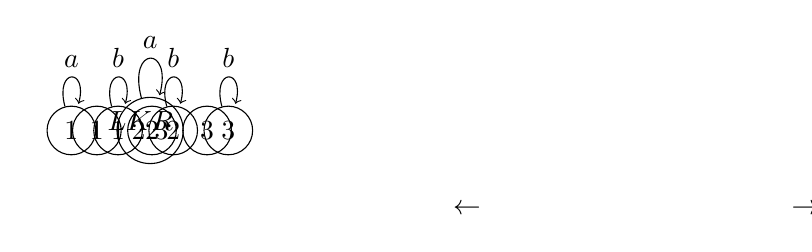
\begin{tikzpicture}[baseline=-10mm]
    \graphbox{$L$}{0mm}{0mm}{38mm}{20mm}{2mm}{-13mm}{
      \node [draw, circle] (x) at (-7mm,0mm) {1};
      \node [draw, circle] (y) at (3mm,0mm) {2 3};
      \draw[->] (x) edge[loop above] node  {$a$} (x);
      \draw[->] (y) edge [loop above] node {$a$} (y);
    }
    \graphbox{$K$}{42mm}{-0mm}{38mm}{20mm}{0mm}{-10mm}{
        \node [draw, circle] (x) at (-7mm,0mm) {1};
        \node [draw, circle] (y) at (0mm,0mm) {2};
        \node [draw, circle] (z) at (7mm,0mm) {3};    
    }
    \begin{scope}[opacity=1]        
    \graphbox{$R$}{85mm}{-0mm}{38mm}{20mm}{2mm}{-13mm}{
      \node [draw, circle] (x) at (-7mm,0mm) {1};
      \node [draw, circle] (y) at (0mm,0mm) {2};
      \node [draw, circle] (z) at (7mm,0mm) {3};
      \draw[->] (x) edge[loop above] node  {$b$} (x);
      \draw[->] (y) edge[loop above] node  {$b$} (y);
      \draw[->] (z) edge[loop above] node  {$b$} (z);
    }
    \end{scope}
    \node () at (40mm,-10mm) {$\leftarrow$};
    \node () at (83mm,-10mm) {$\rightarrow$};
\end{tikzpicture}
}

}
%   \end{center}

%   Its termination is not in the scope of our method due to its non-node-injective left-hand side morphism. 
% \end{example}

% \begin{example}
%   \cite[Example 5.7]{overbeek2024termination_lmcs} has conditions on the host graph, which cannot be modeled by DPO rewriting rules. 
% \end{example}
% \begin{example}
%   The POPO+ rewriting system presented in~\cite[Example 5.7]{overbeek2024termination_lmcs} cannot be modeled by DPO rewriting rules due to the application condition on the context.
%   % Consider Example 5.7  without application condition.

%   % \begin{tikzpicture}
%   %     \graphbox{L}{0mm}{-9mm}{35mm}{8mm}{1mm}{-4mm}{
%   %         \node [draw,circle] (y) at (0mm,0mm) {1};
%   %         \draw [->] (y) edge [loop right] node {} (y);
%   %     }
%   %     \graphbox{K}{36mm}{-9mm}{35mm}{8mm}{1mm}{-4mm}{
%   %         \node [draw,circle] (y) at (0mm,-0mm) {1};
%   %     }
%   %     \begin{scope}[opacity=1]        
%   %         \graphbox{R}{72mm}{-9mm}{35mm}{8mm}{1mm}{-4mm}{
%   %         \node [draw,circle] (y) at (0mm,-0mm) {1};
%   %     }
%   %     \end{scope}
%   %   \end{tikzpicture}

%   % \begin{tikzpicture}
%   %     \graphbox{L}{0mm}{-9mm}{35mm}{8mm}{1mm}{-4mm}{
%   %       \node [draw,circle] (y) at (0mm,0mm) {1};
%   %     }
%   %     \graphbox{K}{36mm}{-9mm}{35mm}{8mm}{1mm}{-4mm}{
%   %     }
%   %     \begin{scope}[opacity=1]        
%   %     \graphbox{R}{72mm}{-9mm}{35mm}{8mm}{1mm}{-4mm}{
%   %     }
%   %     \end{scope}
%   %   \end{tikzpicture}
% \end{example}



% \begin{example}
%   \label{ex:overbeek_5d8_plump1995_3d8_plump2018_3_overbeek_5d8}
%   Consider the DPO rewriting system presented in~\cite[Example 5.8]{overbeek2024termination_lmcs},~\cite[Example 3]{plump2018modular} and~\cite[Example 3.8]{plump1995ontermination}. It rewriting rules are depicted by the bottom spans of the following diagram

% \begin{center}
%  $\rho = ${ 
%   \begin{tikzpicture}[baseline=-20mm]
%         \graphbox{$L$}{0mm}{-11mm}{35mm}{15mm}{0.5mm}{-9mm}{
%           \node [draw, circle] (x) at (-10mm,0mm) {1};
%           \node [draw, circle] (y) at (0mm,0mm) {2};
%           \node [draw, circle] (z) at (10mm,0mm) {3};
%           \draw[->] (x) to node [above] {$a$} (y);
%           \draw[->] (y) to node [above] {$b$} (z);
%         }
%         \graphbox{$K$}{36mm}{-11mm}{35mm}{15mm}{0.5mm}{-9mm}{
%           \node [draw, circle] (x) at (-10mm,0mm) {1};
%           %\node [draw, circle] (y) at (0mm,0mm) {2};
%           \node [draw, circle] (z) at (10mm,0mm) {3};
%         }
%         \begin{scope}[opacity=1]        
%         \graphbox{$R$}{72mm}{-11mm}{35mm}{15mm}{0.5mm}{-9mm}{
%           \node [draw, circle] (x) at (-10mm,0mm) {1};
%           \node [draw, circle] (y) at (0mm,0mm) {2};
%           \node [draw, circle] (z) at (10mm,0mm) {3};
%           \draw[->] (x) to node [above] {$a$} (y);
%           \draw[->] (y) to node [above] {$c$} (z);
%         }
%         \end{scope}
%       \end{tikzpicture}
%  }
% \end{center}

% \begin{center}
%   $\tau = ${ 
%    \begin{tikzpicture}[baseline=-20mm]
%       \graphbox{$L$}{0mm}{-11mm}{35mm}{15mm}{0.5mm}{-9mm}{
%           \node [draw, circle] (x) at (-10mm,0mm) {1};
%           \node [draw, circle] (y) at (0mm,0mm) {2};
%           \node [draw, circle] (z) at (10mm,0mm) {3};
%           \draw[->] (x) to node [above] {$c$} (y);
%           \draw[->] (y) to node [above] {$d$} (z);
%       }
%       \graphbox{$K$}{36mm}{-11mm}{35mm}{15mm}{0.5mm}{-9mm}{
%           \node [draw, circle] (x) at (-10mm,0mm) {1};
%           %\node [draw, circle] (y) at (0mm,0mm) {2};
%           \node [draw, circle] (z) at (10mm,0mm) {3};
%       }
%       \begin{scope}[opacity=1]        
%       \graphbox{$R$}{72mm}{-11mm}{35mm}{15mm}{0.5mm}{-9mm}{
%           \node [draw, circle] (x) at (-10mm,0mm) {1};
%           \node [draw, circle] (y) at (0mm,0mm) {2};
%           \node [draw, circle] (z) at (10mm,0mm) {3};
%           \draw[->] (x) to node [above] {$d$} (y);
%           \draw[->] (y) to node [above] {$b$} (z);
%       }
%       \end{scope}
%       \end{tikzpicture}
%   }
%   \end{center}

%   Let $X$ be  \tikz[baseline=-0.5ex]{
%       \node (x) at (0,0) {$\bullet$};
%       \node (y) at (1,0) {$\bullet$ };
%       \node (z) at (2,0) { $\bullet$};
%       \draw[->] (x) -- (y) node[midway, above] {$a$};
%       \draw[<-] (z) -- (y) node[midway, above] {$b$};
%   } 

%   For both rules, $R_X$ is 

%   \begin{tikzpicture}
%     \graphbox{$R_X$}{36mm}{6mm}{35mm}{15mm}{0.5mm}{-9mm}{
%       % \node [draw, circle] (x) at (-10mm,0mm) {1};
%       % %\node [draw, circle] (y) at (0mm,0mm) {2};
%       % \node [draw, circle] (z) at (10mm,0mm) {3};
%     }
%   \end{tikzpicture}

%   We have 
%   $|\operatorname{Mono}(X,L)| = 1 > 0 = |\operatorname{Mono}(X,R)|$ for $\rho$, and 
%   $|\operatorname{Mono}(X,L)| = 0 = 0 = |\operatorname{Mono}(X,R)|$ for $\tau$, therefore $\rho$ is eliminated.
  
%   Let $Y$ be  \tikz[baseline=-0.5ex]{
%       \node (x) at (0,0) {$\bullet$};
%       \node (y) at (1,0) {$\bullet$ };
%       \draw[->] (x) -- (y) node[midway, above] {$c$};
%   }. For $\tau$, we have

%   \begin{tikzpicture}
%     \graphbox{$R_X$}{36mm}{6mm}{35mm}{15mm}{0.5mm}{-9mm}{
%       % \node [draw, circle] (x) at (-10mm,0mm) {1};
%       % %\node [draw, circle] (y) at (0mm,0mm) {2};
%       % \node [draw, circle] (z) at (10mm,0mm) {3};
%     }
%   \end{tikzpicture} 
  
%   and $|\operatorname{Mono}(Y,L)| = 1 > 0 = |\operatorname{Mono}(Y,R)|$.

%   Thus, this rewriting systems terminates by~\autoref{thm:termination_grs}.
% \end{example}
  
% \begin{example}
%   \label{ex:plump_ex4}
%   Our method cannot prove the termination of the DPO rewriting system with monic matches presented in~\cite[Example 4]{plump2018modular}. The rewriting rules are depicted below
% \begin{center}
%   $r_1 = ${ 
%    \begin{tikzpicture}[baseline=-20mm]
%          \graphbox{$L$}{0mm}{-11mm}{35mm}{15mm}{0.5mm}{-9mm}{
%            \node [draw, circle] (x) at (-10mm,0mm) {1};
%            \node [draw, circle] (y) at (0mm,0mm) {2};
%            \node [draw, circle] (z) at (10mm,0mm) {3};
%            \draw[->] (x) to node [above] {$0$} (y);
%            \draw[->] (y) to node [above] {$L$} (z);
%          }
%          \graphbox{$K$}{36mm}{-11mm}{35mm}{15mm}{0.5mm}{-9mm}{
%            \node [draw, circle] (x) at (-10mm,0mm) {1};
%            %\node [draw, circle] (y) at (0mm,0mm) {2};
%            \node [draw, circle] (z) at (10mm,0mm) {3};
%          }
%          \begin{scope}[opacity=1]        
%          \graphbox{$R$}{72mm}{-11mm}{40mm}{15mm}{-4mm}{-9mm}{
%            \node [draw, circle] (x) at (-10mm,0mm) {1};
%            \node [draw, circle] (y) at (0mm,0mm) {2};
%            \node [draw, circle] (z) at (10mm,0mm) {3};
%            \node [draw, circle] (w) at (20mm,0mm) {3};
%            \draw[->] (x) to node [above] {$L$} (y);
%            \draw[->] (y) to node [above] {$1$} (z);
%            \draw[->] (z) to node [above] {$1$} (w);
%          }
%          \end{scope}
%        \end{tikzpicture}
%   }
%  \end{center}
 
%  \begin{center}
%    $r_2 = ${ 
%     \begin{tikzpicture}[baseline=-20mm]
%        \graphbox{$L$}{0mm}{-11mm}{35mm}{15mm}{0.5mm}{-9mm}{
%            \node [draw, circle] (x) at (-10mm,0mm) {1};
%            \node [draw, circle] (y) at (0mm,0mm) {2};
%            \node [draw, circle] (z) at (10mm,0mm) {3};
%            \draw[->] (x) to node [above] {$R$} (y);
%            \draw[->] (y) to node [above] {$1$} (z);
%        }
%        \graphbox{$K$}{36mm}{-11mm}{35mm}{15mm}{0.5mm}{-9mm}{
%            \node [draw, circle] (x) at (-10mm,0mm) {1};
%            %\node [draw, circle] (y) at (0mm,0mm) {2};
%            \node [draw, circle] (z) at (10mm,0mm) {3};
%        }
%        \begin{scope}[opacity=1]        
%        \graphbox{$R$}{72mm}{-11mm}{35mm}{15mm}{0.5mm}{-9mm}{
%            \node [draw, circle] (x) at (-10mm,0mm) {1};
%            \node [draw, circle] (y) at (0mm,0mm) {2};
%            \node [draw, circle] (z) at (10mm,0mm) {3};
%            \draw[->] (x) to node [above] {$0$} (y);
%            \draw[->] (y) to node [above] {$R$} (z);
%        }
%        \end{scope}
%        \end{tikzpicture}
%    }
%    \end{center}

% \begin{center}
%   $r_3 = ${ 
%    \begin{tikzpicture}[baseline=-20mm]
%          \graphbox{$L$}{0mm}{-11mm}{35mm}{15mm}{0.5mm}{-9mm}{
%            \node [draw, circle] (x) at (-10mm,0mm) {1};
%            \node [draw, circle] (y) at (0mm,0mm) {2};
%            \node [draw, circle] (z) at (10mm,0mm) {3};
%            \draw[->] (x) to node [above] {$B$} (y);
%            \draw[->] (y) to node [above] {$L$} (z);
%          }
%          \graphbox{$K$}{36mm}{-11mm}{35mm}{15mm}{0.5mm}{-9mm}{
%            \node [draw, circle] (x) at (-10mm,0mm) {1};
%            %\node [draw, circle] (y) at (0mm,0mm) {2};
%            \node [draw, circle] (z) at (10mm,0mm) {3};
%          }
%          \begin{scope}[opacity=1]        
%          \graphbox{$R$}{72mm}{-11mm}{35mm}{15mm}{0.5mm}{-9mm}{
%            \node [draw, circle] (x) at (-10mm,0mm) {1};
%            \node [draw, circle] (y) at (0mm,0mm) {2};
%            \draw[->] (x) to node [above] {$R$} (y);
%          }
%          \end{scope}
%        \end{tikzpicture}
%   }
%  \end{center}
 
%  \begin{center}
%    $r_4 = ${ 
%     \begin{tikzpicture}[baseline=-20mm]
%        \graphbox{$L$}{0mm}{-11mm}{35mm}{15mm}{0.5mm}{-9mm}{
%            \node [draw, circle] (x) at (-10mm,0mm) {1};
%            \node [draw, circle] (y) at (0mm,0mm) {2};
%            \node [draw, circle] (z) at (10mm,0mm) {3};
%            \draw[->] (x) to node [above] {$R$} (y);
%            \draw[->] (y) to node [above] {$B$} (z);
%        }
%        \graphbox{$K$}{36mm}{-11mm}{35mm}{15mm}{0.5mm}{-9mm}{
%            \node [draw, circle] (x) at (-10mm,0mm) {1};
%            %\node [draw, circle] (y) at (0mm,0mm) {2};
%            \node [draw, circle] (z) at (10mm,0mm) {3};
%        }
%        \begin{scope}[opacity=1]        
%        \graphbox{$R$}{72mm}{-11mm}{35mm}{15mm}{0.5mm}{-9mm}{
%            \node [draw, circle] (x) at (-10mm,0mm) {1};
%            \node [draw, circle] (y) at (0mm,0mm) {2};
%            \node [draw, circle] (z) at (10mm,0mm) {3};
%            \draw[->] (x) to node [above] {$L$} (y);
%            \draw[->] (y) to node [above] {$B$} (z);
%        }
%        \end{scope}
%        \end{tikzpicture}
%    }
%    \end{center}

%   The rule $r_3$ can be eliminated by considering monomorphisms from  \tikz[baseline=-0.5ex]{
%     \node (x) at (0,0) {$\bullet$};
%     \node (y) at (1,0) {$\bullet$ };
%     \draw[->] (x) -- (y) node[midway, above] {$B$};
%   }, then the rule $r_4$ can be eliminated by considering monomorphisms from  \tikz[baseline=-0.5ex]{
%   \node (x) at (0,0) {$\bullet$};
%   \node (y) at (1,0) {$\bullet$ };
%   \draw[->] (x) -- (y) node[midway, above] {$R$};
% }.

% But our method cannot eliminate $r_1$ and $r_2$. However, combined with the technique proposed by Plump in~\cite{plump2018modular}, we can prove the termination of this rewriting system: $\{r_1\}$ and $\{r_2\}$ are both terminating, and their union is terminating by~\cite{plump2018modular}.
% \end{example}

% \begin{example}
%   \label{ex:bruggink2015_ex5}
%   Our method cannot prove the termination of the DPO rewriting system with monic matches presented in~\cite[Example 5]{bruggink2015proving}. 
% \end{example}
% \begin{example}
%   \label{ex:bruggink2015_ex6_endrullis2024_d2}
%   Our method cannot prove the termination of the DPO rewriting system with monic matches presented in~\cite[Example 6]{bruggink2015proving}. 
% \end{example}

% \begin{example}
%   \label{ex:plump2018_ex6_endrullis_d4}
%   The DPO rewriting system with monic matches presented in~\cite[Example 6]{plump2018modular} is not in the scope of our method due to the non-injective rule.
% \end{example}


% \begin{example} 
%   \label{ex:termination:contrib} 
%   The rewriting rule illustrated below is from~\cite[Example 6]{plump2018modular}.
%   % \begin{figure}[H] 
%   \begin{center}
%     $\tau = ${ \resizebox{0.6\textwidth}{!}{
%       \begin{tikzpicture}[baseline=-17mm]
%           \graphbox{$L$}{0mm}{0mm}{35mm}{35mm}{2mm}{-5mm}{
%               \coordinate (delta) at (0,-18mm);
%               \node[draw,circle] (l1) at ($(delta) + (-1,1.5)$) {1};
%               \node[draw,circle] (l2) at ($(delta) + (1,1.5)$) {2};
%               \node[draw,circle] (l3) at ($(delta) + (0,0)$) {3};
%               \draw[->] (l1) -- (l3) node[midway,left] {s};
%               \draw[->] (l2) -- (l3) node[midway,right] {s};
%               \draw[->] (l3) edge [loop below] node {0} (l3);
%           }
%           \graphbox{$K$}{40mm}{0mm}{35mm}{35mm}{2mm}{-5mm}{
%               \coordinate (delta) at (0,-18mm);
%               \coordinate (interfaceorigin) at ($(delta) +(5,0)$);
%               \node[draw,circle] (r1) at ($(delta) +(-1,1.5)$) {1};
%               \node[draw,circle] (r2) at ($(delta) +(0.5,1.5)$) {2};
%               \node[draw,circle] (r3) at ($(delta) + (0,0)$) {3};
%               \draw[->] (r1) -- (r3) node[midway,left] {s};
%               \draw[->] (r3) edge [loop below] node {0} (r3);
%           }
%           \graphbox{$R$}{80mm}{0mm}{35mm}{35mm}{2mm}{-5mm}{
%               \coordinate (delta) at (0,-18mm);
%               \node[draw,circle] (r1) at ($(delta) + (-1,1.5)$) {1};
%               \node[draw,circle] (r2) at ($(delta) + (0.5,1.5)$) {2};
%               \node[draw,circle] (r3) at ($(delta) + (0,0)$) {3};
%               \node[draw,circle] (r4) at ($(delta) + (1,0)$) {};
%               \draw[->] (r1) -- (r3) node[midway,left] {s};
%               \draw[->] (r2) -- (r4) node[midway,right] {s};
%               \draw[->] (r4) edge [loop below] node {0} (r4);
%               \draw[->] (r3) edge [loop below] node {0} (r3);
%           }
%           % \graphbox{$R_x$}{40mm}{40mm}{35mm}{35mm}{2mm}{-5mm}{
%           %     \coordinate (delta) at (0,-18mm);
%           %     \coordinate (rxorigin) at ($(interfaceorigin)+(0,6)$);
%           %     \node[draw,circle] (r1) at ($(delta) + (-1,1.5)$) {1};
%           %     \node[draw,circle] (r2) at ($(delta) +  (0.5,1.5)$) {2};
%           %     \node[draw,circle] (r3) at ($(delta) +  (0,0)$) {3};
%           %     \draw[->] (r1) -- (r3) node[midway,left] {s};
%           %     \draw[->] (r3) edge [loop below] node {0} (r3);
%           % }
%           \node () at (37mm,-18mm) {$\leftarrowtail$};
%           \node () at (78mm,-18mm) {$\rightarrowtail$};
%           % \node () at (57mm,2mm) {$\uparrowtail$};
%           % \node () at (38mm,2mm) {$\swarrowtail$};
%           % \node () at (79mm,2mm) {$\searrowtail$};
%       \end{tikzpicture}
%       }
%     }
%   \end{center}
%   Its termination can be proved by our method.
% \end{example}  

% \begin{example}
%   \label{ex_endrullis_6d3_endrullis_5d8}
%   Consider the rule presented in~\cite[Example 6.3]{endrullis2024generalized_arxiv_v2} illustrated in the bottom span of the following diagram:
%   % \begin{figure}[H] 
%   %     \center
%   \begin{center}
%       \resizebox{0.6\textwidth}{!}{
%           \begin{tikzpicture}
%               \graphbox{$L$}{0mm}{0mm}{35mm}{25mm}{2mm}{-8mm}{
%                   \coordinate (delta) at (0,-18mm);
%                   \node[draw,circle] (x) at (-6mm,-10mm) {x};
%                   \node[draw,circle] (y) at (6mm,-10mm) {y};
%                   \node[draw,circle]  (z) at (6mm,0mm) {z};
%                   \draw[->]  (x) to (y);
%                   \draw[->] (y) to[bend right=20] (z);
%                   \draw[->]  (z) to[bend right=20] (y);
%               }
%               \graphbox{$K$}{40mm}{0mm}{35mm}{25mm}{2mm}{-8mm}{
%                   \node[draw,circle]  (x) at (-6mm,-10mm) {x};
%                   \node[draw,circle]  (y) at (6mm,-10mm) {y};
%               }
%               \graphbox{$R$}{80mm}{0mm}{35mm}{25mm}{2mm}{-8mm}{
%                   \node[draw,circle]  (x) at (-6mm,-10mm) {x};
%                       \node[draw,circle]  (y) at (6mm,-10mm) {y};
%                       \node[draw,circle]  (z) at (0mm,0mm) {w};
%                       \draw[->]  (x) to (y);
%                       \draw[->]  (y) to [bend left=0] (z);
%                       \draw[->]  (z) to [bend left=0] (x);
%               }
%               \graphbox{$R_x$}{40mm}{20mm}{35mm}{15mm}{2mm}{2mm}{
%                   \node[draw,circle]  (x) at (-6mm,-10mm) {x};
%                   \node[draw,circle]  (y) at (6mm,-10mm) {y};
%                   \draw[->]  (x) to (y);
%               }
%               \node () at (37mm,-12mm) {$\leftarrowtail$};
%               \node () at (78mm,-12mm) {$\rightarrowtail$};
%               \node () at (57mm,2mm) {$\uparrowtail$};
%               \node () at (38mm,2mm) {$\swarrowtail$};
%               \node () at (79mm,2mm) {$\searrowtail$};
%           \end{tikzpicture}
%       }
%   \end{center}

%   Let $X$ be the graph 
%   \tikz[baseline=-0.5ex]{
%       \node (x) at (0,0) {$\bullet$};
%       \node (y) at (1,0) {$\bullet$};
%       \draw[->] (x) to[bend right=20] (y);
%       \draw[->] (y) to[bend right=20] (x); 
%   } and $\mathbb{X} = \{X\}$. Let $s_\mathbb{X}$ be the weight function associating the weight of $1$ to $X$. There is only one element 
%   \scalebox{0.7}{\tikz[baseline=-0.5ex]{
%           \node [draw,circle] (x) at (0,0) {x};
%           \node[draw,circle] (y) at (1,0) {y};
%           \draw[->] (x) -- (y) node[midway, above] {};
%       }}
%   in $D(X, R)$. 
%    Since $w_{s_\mathbb{X}}(L) = 1 > 0 = w_{s_\mathbb{X}}(R)
%       $, the rule terminates by~\autoref{thm:termination_grs}.
% \end{example}


% \begin{example}[Limitation]
%   \label{ex:plump95_4d1}
%  Consider a rule presented in~\cite[Example 4.1]{plump1995ontermination}:

%   \begin{center}
%       \resizebox{0.7\textwidth}{!}{
%     $\rho = $  \begin{tikzpicture}[baseline=-20mm]
%       \graphbox{$L$}{0mm}{0}{32mm}{40mm}{0}{0}{
%           \node[draw,circle]  (n1) at (0,-6mm) {1};
%           \node[draw,circle]   (n2) at (0mm,-26mm) {2};
%           \node[draw,circle]   (n3) at (-10mm,-26mm) {3};
%           \node[draw,circle]   (n4) at (10mm,-26mm) {4};
%           \draw[->]  (n2) edge [loop below] node  {a} (n2);
%           \draw[->]  (n3) edge [loop below] node  {b} (n3);
%           \draw[->]  (n1) to node [right] {f} (n2) ;
%           \draw[->]  (n1) to node [right] {f}  (n3);
%           \draw[->]  (n1) to node [right] {f}  (n4);
%         }
%         \graphbox{$K$}{33mm}{0}{32mm}{40mm}{0}{-0}{
%           \node[draw,circle]  (n1) at (0,-6mm) {1};
%           \node[draw,circle]   (n2) at (0mm,-26mm) {2};
%           \node[draw,circle]   (n3) at (-10mm,-26mm) {3};
%           \node[draw,circle]   (n4) at (10mm,-26mm) {4};
%           \draw[->]  (n2) edge [loop below] node  {a} (n2);
%           \draw[->]  (n3) edge [loop below] node  {b} (n3);
%         }
%         \graphbox{$R$}{66mm}{0}{32mm}{40mm}{0}{-0}{
%           \node[draw,circle]  (n1) at (0,-6mm) {1};
%           \node[draw,circle]   (n2) at (0mm,-26mm) {2};
%           \node[draw,circle]   (n3) at (-10mm,-26mm) {3};
%           \node[draw,circle]   (n4) at (10mm,-26mm) {4};
%           \draw[->]  (n2) edge [loop below] node  {a} (n2);
%           \draw[->]  (n3) edge [loop below] node  {b} (n3);
%           \draw[->]  (n1) edge [bend left] node [right] {f} (n4) ;
%           \draw[->]  (n1) edge [bend right] node [left] {f}  (n4);
%           \draw[->]  (n1) to node [right] {f}  (n4);
%         }   
%   \end{tikzpicture}
%       }
% \end{center}
% \noindent
% \begin{minipage}{0.7\textwidth}
%   To prove its termination with our method, a ruler-graph $X$ containing an edge labeled by $f$ must be used, because the number of occurrences of every graph containing only edges labeled by $a$ and $b$ does not change by any rewriting step using $\rho$. But in this case, condition~\eqref{def:non_increasing_rule_img_edges_distinct} of~\autoref{def:creates_more_x_on_the_left} cannot be satisfied.
% \end{minipage}
% \begin{minipage}{0.3\textwidth}
%   \hfill
% \begin{center}
%   \begin{tikzpicture} 
%       \graphbox{}{0}{0}{30mm}{20mm}{-10mm}{-10mm}{
%           \node[draw,circle]  (n1) at (0,0mm) {1};
%           % \node[draw,circle]   (n2) at (0mm,-26mm) {2};
%           % \node[draw,circle]   (n3) at (-10mm,-26mm) {3};
%           \node[draw,circle]   (n4) at (20mm,0mm) {4};
%           % \draw[->]  (n2) edge [loop below] node  {a} (n2);
%           % \draw[->]  (n3) edge [loop below] node  {b} (n3);
%           \draw[->]  (n1) edge [bend left] node [above] {f} (n4) ;
%           \draw[->]  (n1) edge [bend right] node [below] {f}  (n4);
%           \draw[->]  (n1) to node {f}  (n4);
%         }  
%   \end{tikzpicture}
% \end{center}
% \end{minipage}

% \end{example}

% \begin{example}
%   \label{ex:termination:grsaa}
%   Consider the rewriting rule in~\autoref{ex:grsaa_rx}. Let $X$ be the graph \tikz[baseline=-0.5ex]{
%       \node (x) at (0,0) {$\bullet$};
%       \node (y) at (1,0) {$\bullet$ }; 
%       \node (z) at (2,0) { $\bullet$};
%       \draw[->] (x) -- (y) node[midway, above] {$a$};
%       \draw[<-] (z) -- (y) node[midway, above] {$a$};
%   } with weight $1$ and $\mathbb{X} = \{X\}$. The rule is $X$-non-increasing by~\autoref{example:grs_aa:has_more_left}. 
%   % Let $s_\mathbb{X}$ be the weight function which associates the weight of $1$ to $X$. 
%   % Since \(w_{s_\mathbb{X}}(L) = 1 > 0 = w_{s_\mathbb{X}}(R)\), 
%   Since \(w(L) = 1 > 0 = w(R)\),
%   it terminates by~\autoref{thm:termination_grs}.
% \end{example}

% We present an example where $\mathbb{X}$ is not a singleton.
% \begin{example} 
%   \label{ex:overbeek_5d6}
%   Consider the rewriting rules presented in~\cite[Example 5.6]{overbeek2024termination_lmcs} illustrated below:
%   \begin{center}
%     $\rho = $\scalebox{0.7} { {
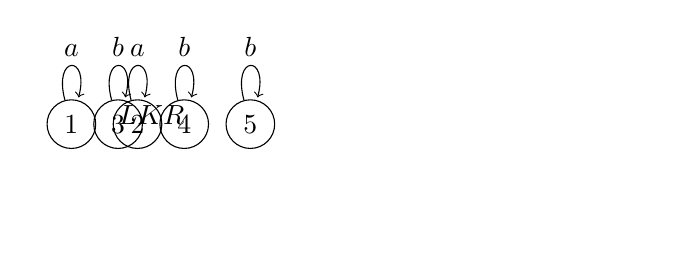
\begin{tikzpicture}[baseline=-15mm,scale=1.2]
    \graphbox{$L$}{0mm}{0mm}{31mm}{20mm}{2mm}{-13mm}{
      \node [draw, circle] (x) at (-7mm,0mm) {1};
      \node [draw, circle] (y) at (0mm,0mm) {2};
      \draw[->] (x) edge[loop above] node  {$a$} (x);
      \draw[->] (y) edge [loop above] node {$a$} (y);
    }
    \graphbox{$K$}{35mm}{-0mm}{18mm}{20mm}{0mm}{-10mm}{
    }
    \begin{scope}  
    \graphbox{$R$}{57mm}{-0mm}{38mm}{20mm}{2mm}{-13mm}{
      \node [draw, circle] (x) at (-7mm,0mm) {3};
      \node [draw, circle] (y) at (0mm,0mm) {4};
      \node [draw, circle] (z) at (7mm,0mm) {5};
      \draw[->] (x) edge[loop above] node  {$b$} (x);
      \draw[->] (y) edge[loop above] node  {$b$} (y);
      \draw[->] (z) edge[loop above] node  {$b$} (z);
    }
    \end{scope}
    \node () at (33mm,-12mm) {$\leftarrowtail$};
    \node () at (55mm,-12mm) {$\rightarrowtail$};
\end{tikzpicture}
}}
%   \end{center}
%   \begin{center}
%   $\tau = $\scalebox{0.7}{ {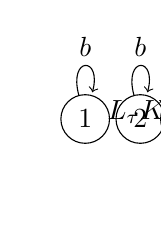
\begin{tikzpicture}[baseline=-10mm]
    \graphbox{$L_\tau$}{0mm}{0}{31mm}{20mm}{2mm}{-13mm}{
        \node[draw,circle] (x) at (-7mm,0mm) {1};
        \node[draw,circle] (y) at (0mm,0mm) {2};
        \draw[->] (x) edge[loop above] node {$b$} (x);
        \draw[->] (y) edge [loop above] node {$b$} (y);
      }
      \graphbox{$K_\tau$}{32mm}{0}{18mm}{20mm}{2mm}{-13mm}{
      }
      \begin{scope}[opacity=1]        
      \graphbox{$R_\tau$}{51mm}{0}{25mm}{20mm}{1mm}{-13mm}{
        \node[draw,circle] (x) at (-3.5mm,0mm) {3};
        \draw[->] (x) edge[loop above] node {$a$} (x);
      }
      \end{scope}
  \end{tikzpicture}}
%   }
%   \end{center}
%   Let $X$ be 
%   \tikz[baseline=-0.5ex]{
%       \node (x) at (0,0) {$\bullet$};
%       \draw[->] (x) edge [loop right] node {a} (x);
%   } with weight $5$, let $Y$ be
%   \tikz[baseline=-0.5ex]{
%       \node (x) at (0,0) {$\bullet$};
%       \draw[->] (x) edge [loop right] node {b} (x);
%   } with weight $3$ and $\mathbb{X} = \{X, Y\}$.
%   The rules $\rho$ and $\tau$ are both $X$- and $Y$-non-increasing with $D(rhs(\rho), X) = D(rhs(\rho), Y) = D(rhs(\tau), X) = D(rhs(\tau), Y) = \emptyset$.   
%   % Let $s_\mathbb{X}$ be the weight function associating the weight of $5$ to $X$ and the weight of $3$ to $Y$.
%   % We have $
%   %     w_{s_\mathbb{X}}(\operatorname{lhs}(\rho)) = 10 > 9 = w_{s_\mathbb{X}}(\operatorname{rhs}(\rho))
%   %     $ and $
%   %     w_{s_\mathbb{X}}(\operatorname{lhs}(\tau)) = 6 > 5 = w_{s_\mathbb{X}}(\operatorname{rhs}(\tau))$.
%   We have $
%   w(\operatorname{lhs}(\rho)) = 10 > 9 = w(\operatorname{rhs}(\rho))
%   $ and $
%   w(\operatorname{lhs}(\tau)) = 6 > 5 = w(\operatorname{rhs}(\tau))$.
%   Thus, this rewriting systems terminates by~\autoref{thm:termination_grs}.
% \end{example}